\documentclass[a4paper,12pt]{article}
\usepackage{polski}
\usepackage[utf8]{inputenc}
\usepackage[OT4]{fontenc}
\usepackage{mathtools}
\usepackage{float}
\usepackage{graphicx}
\usepackage{multirow}

\newcommand{\h}[1]{\noindent \bf #1 \rm \\ \noindent}
\newcommand{\italic}[1]{\it #1 \rm}


\begin{document}

\begin{center}
	\LARGE
	Sieci Komputerowe \\
	\large
	LABORATORIUM 1 
\end{center}
\vspace{1cm}
	
\h{Komenda "ipconfig":}
Komenda pozwalająca na wyświetlenie danych nt konfiguracji sieciowej komputera lub jej zmianę. Może one być użyta chociażby do sprawdzenia aktualnie przypisanego urządzeniu adresu IPv4. Na systemach UNIX jej odpowiednikiem jest \it ifconfig\rm.

\begin{figure}[H]
	\centering
	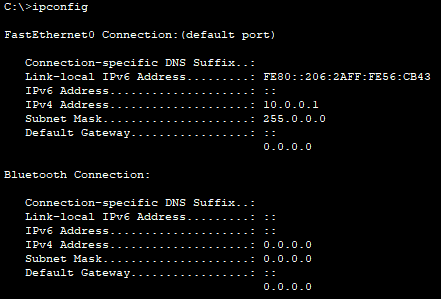
\includegraphics[width=10cm]{fig1.png}
	\caption{Efekt skorzystania z komendy \it ipconfig\rm.}
\end{figure}

\noindent
Do komendy \it ipconfig \rm możemy dodać również parametry, zmieniające jej działanie:
\begin{itemize}
	\item \italic{brak parametru} - wyświetlenie skrótowej informacji nt konfiguracji sieciowej
	\item \italic{/all} - wyświetla szczegółowe informacje na temat konfiguracji sieciowej (w tym adres MAC)
	\item \italic{/release} - zwalnia wszystkie adresy IP przydzielone do karty sieciowej
	\item \italic{/renew} - pobiera nowe adresy IP dla karty sieciowej (wymaga aktywnego DHCP)
	\item \italic{/flushdns} - usuwa informacje na temat nazw domen z pamięci serwera DNS 
	\item \italic{displaydns} - wyświetla nazwy domen zawarte w pamięci serwera DNS
	\item \italic{registerdns} - odświeża i aktualizuje informacje o nazwach domen w serwerze DNS
\end{itemize}

\h{Komenda "ping":}
Komenda pozwalająca na diagnozowanie połączenia sieciowego między dwoma urządzeniami w sieci. Badanie polega na przesłaniu kolejno 4 pakietów ICMP z jednego urządzenia i oczekiwanie na odpowiedź z drugiego. Czas między wysłaniem pakietu a otrzymaniem odpowiedzi nazywamy czasem odpowiedzi czy też czasem ping.
	
\begin{figure}[H]
	\centering
	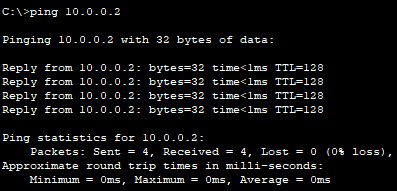
\includegraphics[width=10cm]{fig2.png}
	\caption{Efekt skorzystania z komendy \it ping\rm.}
\end{figure}	

\noindent
Za pomocą parametrów można dostosować ilość wysyłanych pakietów, czas oczekiwania na odpowiedź oraz rozmiar pakietów. Najczęściej używanymi są:
\begin{itemize}
	\item \italic{-n [ilość]} - ustala ilość pakietów które mają zostać przesłane
	\item \italic{-l [ilość]} - ustala wielkość pakietów
	\item \italic{-w [czas msek]} - określa maksymalny czas oczekiwania na odpowiedź
	\item \italic{-a} - nastąpi próba identyfikacji nazwy z serwera DNS
\end{itemize}

\noindent
Zamiast adresu IPv4 odbiorcy mnożna wpisać nazwę hosta, która następnie zostanie rozpoznana przez DNS.\\

\h{Protokół ICMP:}
Protokół ICMP (Internet Control Message Protocol) to protokół warstwy sieciowej, który jest używany do przesyłania wiadomości diagnostycznych i sterujących w sieciach IP. Często jest stosowany w diagnozowaniu problemów z siecią. Jego działanie polega na przesyłaniu wiadomości ICMP z między hostami, a następnie oczekiwaniu na odpowiedź.\\

\h{Komenda "tracert":}
Komenda pozwalająca na prześledzenie ścieżki pomiędzy hostami. Wyświetli ona informacje o wszystkich routerach przez które należy przejść, aby dotrzeć do hosta (pokaże dane o ścieżce do hosta). Jest to narzędzie oparte o wiadomości ICMP. Pozwala ono ustalić w łatwy sposób w którym punkcie ścieżki występuje problem z transmisją.

\begin{figure}[H]
	\centering
	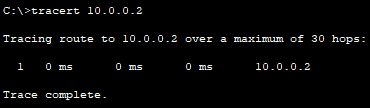
\includegraphics[width=10cm]{fig3.png}
	\caption{Efekt skorzystania z komendy \it tracert\rm.}
\end{figure}

Do komendy \italic{tracert} można dodać parametr zmieniający jej działanie:
\begin{itemize}
	\item \italic{-d} - wyłącza konwersję adresów na nazwy hostów (DNS).
	\item \italic{-h [ilość]} - ustala maksymalną ilość skoków, z których ma składać się ścieżka
\end{itemize}

\h{Host:}
Każde urządzenie podłączone do sieci, które bierze bezpośredni udział w komunikacji sieciowej (jest urządzeniem końcowym). Każdy host obecny ma przypisany numer identyfikacyjny, adres IP (zgodny ze schematem adresowania protokołu IP).\\

\h{Serwery i klienci}
Wśród hostów można wyróżnić urządzenia będące serwerami i klientami. Serwery posiadają oprogramowanie umożliwiające im dostarczanie informacji klientom danej usługi sieciowej. Urządzenia-klienci posiadają oprogramowanie do wysyłania żądań i wyświetlania danych przychodzących z serwerów. Oczywiście nic nie stoi na przeszkodzie, aby urządzenie było jednocześnie klientem jak i serwerem (chodź zazwyczaj taka sytuacja nie występuje).\\

\h{Sieć peer-to-peer:}
O sieci peer-to-peer mówimy, gdy występujące w sieci hosty pełnią rolę zarówno klienta jak i serwera. Tego typu sieci występują chociażby w domach czy małych firmach.
\begin{figure}[H]
	\centering
	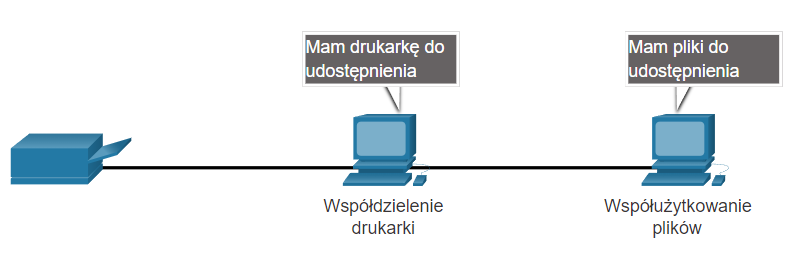
\includegraphics[width=10cm]{fig4.png}
	\caption{Schemat obrazujący sieć peer-to-peer.}
\end{figure}

\noindent
Plusami sieci pper-to-peer są:
\begin{itemize}
	\item Łatwa konfiguracja
	\item Mała złożoność
	\item Niższy koszt ze względu na brak wymogu zakupu dedykowanych urządzeń sieciowych i serwerów
	\item Duża użyteczność w wypadku prostych zadań jak współdzielenie plików i urządzeń wyjścia między urządzeniami
\end{itemize}
\vspace{5mm}

\noindent
Minusami sieci peer-to-peer są:
\begin{itemize}
	\item Brak scentralizowanej administracji (brak centralnego urządzenia-serwera).
	\item Mniejsze bezpieczeństwo 
	\item Trudna skalowalność
	\item Zmniejszona wydajność ze względu na fakt, że każde urządzenie musi wykonywać zadania hosta i serwera
\end{itemize}
\vspace{5mm}

\h{Urządzenia pośredniczące:}
Urządzenia łączące poszczególne urządzenia końcowe z siecią. Ponadto mogą łączyć wiele pojedynczych sieci. Tworzą tym samym intersieć. Urządzenia pośredniczące używają adresy urządzeń końcowych oraz informacje nt połączeń wewnątrz sieci w celu określenia ścieżki, którą powinny obrać wiadomości transmitowane w sieci.\\

\noindent
Odpowiedzialnością urządzeń pośredniczących jest:
\begin{itemize}
	\item Regeneracje i retransmisja sygnałów komunikacyjnych (zawsze).
	\item Utrzymywanie danych nt istniejących w sieci ścieżkach transmisyjnych
	\item Powiadamianie innych urządzeń o błędach i awariach w komunikacji
	\item Przekierowywanie danych alternatywną ścieżką w wypadku awarii łącza
	\item Klasyfikacja i kierowanie wiadomościami zgodnie z priorytetami
	\item Blokowanie lub umożliwianie przepływu danych zgodnie z ustawieniami bezpieczeństwa
\end{itemize}
\vspace{5mm}

\noindent
Urządzeniami pośredniczącymi są:
\begin{itemize}
	\item Routery przewodowe lub bezprzewodowe
	\item Przełączniki (switch) sieci LAN
	\item Przełączniki wielowarstwowe 
	\item Zapory ogniowe (firewall)
\end{itemize}
\vspace{5mm}

\h{Medium sieciowe:}
Komunikację miedzy urządzeniami w sieci zapewniają media sieciowe. To właśnie one tworzą kanały, które służą do przesyłania wiadomości od źródła do celu. W nowoczesnych sieciach komunikacja odbywa się za pomocą mediów takich jak:
\begin{itemize}
	\item \italic{Przewody metalowe} - przesył danych w formie impulsów elektrycznych
	\item \italic{Kable światłowodowe} - przesył danych w formie impulsów świetlnych
	\item \italic{Transmisja bezprzewodowa} - przesył danych za pomocą fal elektromagnetycznych
\end{itemize}
\vspace{5mm}

Kryteria doboru medium sieciowego to:
\begin{itemize}
	\item Odległość na jaką medium może poprawnie transmitować sygnał
	\item Otoczenie, w którym medium ma zostać zainstalowane
	\item Ilość danych, którą medium ma transmitować i prędkość tej transmisji 
	\item Koszt danego medium i jego instalacji
\end{itemize}

\h{Karta sieciowa:}
Moduł umożliwiające fizyczne połączenie urządzenia końcowego z siecią.\\

\h{Port fizyczny:}
Wtyczka/gniazdo w urządzeniu sieciowym, do którego podłączone jest medium łączące to urządzenie z innym urządzeniem sieciowym.\\

\h{Interfejs:}
Specjalny port w urządzeniu sieciowym, który zapewnia połączenie z innymi sieciami. W routerach (urządzeniach służących do łączenia sieci) porty nazywamy interfejsami sieciowymi.\\

\h{Schemat topologii fizycznej:}
Schemat przedstawiający fizyczne położenie urządzeń i mediów w sieci.
\begin{figure}[H]
	\centering
	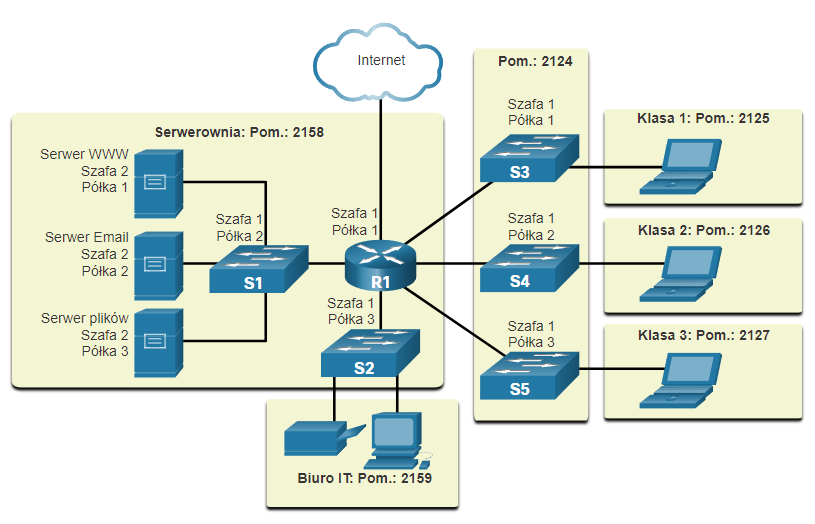
\includegraphics[width=9cm]{fig5.png}
	\caption{Schemat przedstawiający topologię fizyczną sieci.}
\end{figure}

\h{Schemat topologii logicznej:}
Schemat przedstawiający urządzenia, porty i schemat adresowania sieci.
\begin{figure}[H]
	\centering
	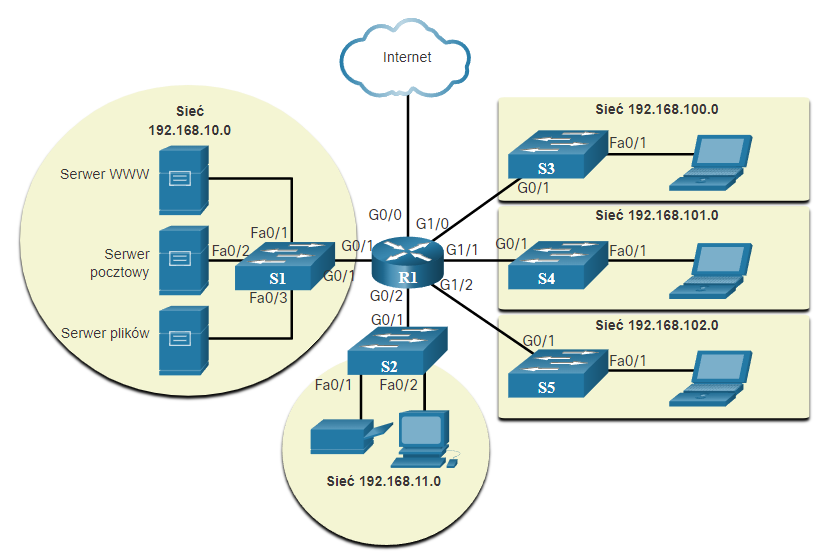
\includegraphics[width=9cm]{fig6.png}
	\caption{Schemat przedstawiający topologię logiczną sieci.}
\end{figure}
\vspace{5mm}

\h{Sieć LAN:}
Sieć lokalna (Local Area Network), rozpościerająca się na małym obszarze geograficznym. Może być to np. sieć łącząca urządzenia na obszarze jednego gospodarstwa domowego. Jest ona administrowana przez jedną organizację/osobę. Zapewnia ona wysoką przepustowość do wewnętrznych urządzeń sieciowych.\\

\h{Sieć WAN:}
Sieć Wide Area Network, rozpościerająca się na dużym obszarze geograficznym. Jest to sieć łącząca ze sobą poszczególne sieci LAN. Jest administrowana przez kilku usługodawców internetowych (ISP, Internet Service Provider). Typowo zapewniają wolne połączenie między połączonymi przez WAN sieciami LAN.\\

\h{Internet:}
Ogólnoświatowy zbiór połączonych ze sobą sieci. Może być zinterpretowany jako grupa połączony ze sobą sieci LAN i WAN. Internet nie jest niczyją własnością. Istnieją jednak organizacje, które zajmują się monitorowaniem struktury i standardów globalnej sieci.\\

\h{Intranet:}
Prywatne połączenie sieciowe należące do jakiejś organizacji. Dostępny tylko dla członków tej organizacji lub innych osób, które uzyskały autoryzację.\\

\h{Ekstranet:}
Siec wykorzystywana przez organizację w celu zapewnienia dostępu swoim współpracownikom czy też klientom do swoich danych. Przykładem jest ekstranet szpitala, który zapewnia dostęp do systemu rezerwacji wizyt online dla pacjentów.\\

\h{Połączenie internetowe dla osób prywatnych i małych firm:}
W wypadku gospodarstw domowych i małych firm połączenie z internetem odbywa się za pomocą:
\begin{itemize}
	\item \italic{Łącza kablowego} - połączenie przez kabel telewizji kablowej o wysokiej przepustowości i dostępności.
	\item \italic{DSL (Digital Subscriber Line)} - połączenie przez linie telefoniczne o wysokiej przepustowości i dostępności. Często dostępne w formie ADSL, gdzie prędkość pobierania jest większa od prędkości przesyłu.
	\item \italic{Sieci komórkowej} - połączenie bezprzewodowe uzależnione od dostępności sygnału sieci komórkowej.
	\item \italic{Satelity} - połączenie bezprzewodowe poprzez sygnał satelitarny, wymagające bezpośredniej widoczności z satelitą.
	\item \italic{Łącze telefoniczne dial-up} - tanie połączenie poprzez linie telefoniczną i modem o niskiej przepustowości.
\end{itemize}
\vspace{5mm}

\h{Połączenie internetowe dla dużych organizacji:}
Ze względu na większe wymagania co do przepustowości i dostępności pasma duże organizacje mają swoje własne metody połączenia z internetem:
\begin{itemize}
	\item \italic{Dedykowane łącza dzierżawione} - wynajmowane przez organizacje dedykowane obwody zapewniające połączenie między biurami.
	\item \italic{Metro Ethernet} - połączenie przewodowe rozszerzające technologię dostępu LAN na sieci WAN.
	\item \italic{Biznes DSL} - połączenie poprzez linie telefoniczne o wysokiej wydajności i dostępności o równych prędkościach przesyłu i pobierania (SDSL). 
	\item \italic{Satelita} - połącznie bezprzewodowe poprzez satelitę.
\end{itemize}
\vspace{5mm}

\h{Sieci konwergentne:}
Sieci będące w stanie transportować wiele usług (dane, wideo, audio itd) poprzez jedną i ta samą sieć. Każda z tych przesyłanych usług podlega pod te same reguły, standardy i umowy. \\

\h{Aspekty niezawodności sieci:}
Nowoczesne sieci są projektowane z zachowaniem odpowiednich standardów, które zapewniają jej poprawne i wydajne funkcjonowanie. Architekci projektując sieć skupiają swoją uwagę na czterech askeptach:
\begin{itemize}
	\item tolerancji błędu
	\item skalowalności
	\item jakości usług(QoS, Quality of Service)
	\item bezpieczeństwie
\end{itemize}
\vspace{5mm}

\h{Tolerancja błędu:}
Sieci powinny być odporne na awarie, czyli w stworzone w sposób ograniczający liczbę urządzeń, które zostaną dotknięte niedogodnościami w wypadku awarii. Muszą być zbudowane tak, aby w wypadku wystąpienia awarii istniał łatwy sposób na odzyskanie sprawności sieci. W tym celu korzystają one z tzw. ścieżek nadmiarowych, które mogą zastąpić uszkodzone ścieżki (sieci z nadmiarowością).\\

\noindent
Routery są w stanie wykorzystywać nadmiarowość wykorzystując przełączanie pakietów. Każda wiadomość w sieci jest dzielona na części zwane pakietami, które oprócz właściwych danych zawierają dodatkowe informacje w swoim nagłówku. Następnie każdy pakiet jest osobno przesyłany do odbiorcy końcowego. Router przy każdym kolejnym pakiecie dynamicznie dobiera ścieżkę. Oznacza to, że każdy pakiet danej wiadomości może zostać de facto przesłany inną ścieżką.\\

\h{Skalowalność:}
Sieć musi być skalowalna, aby w prosty sposób móc obsługiwać coraz to nowych użytkowników i aplikacje. Skalowalność zakłada, że takie rozszerzenie odbywa się bez uszczerbku na wydajności już istniejących w sieci usług (inni użytkownicy nie mogą być poszkodowani tym, że podłączyliśmy nowe urządzenie). Skalowalność można osiągnąć przestrzegając przyjętych ogólnie standardów i protokołów.\\

\h{Jakość usług:}
Nowoczesne sieci są konwergentne, są w stanie przysyłać wiele różnych typów informacji. W wypadku przepełnienia łącza w celu zapewnienia dobrej jakości usług sieciowych routery są w stanie priorytetyzować transport jednego typu danych nad drugim (np. przesył głosu ma priorytet nad przesyłem danych, bo niestabilna transmisja w połączeniu głosowym jest bardziej uciążliwa niż w wypadku chociażby otwierania stron WWW). Takie priorytety są ustalane w polityce jakości usług.\\

\h{Bezpieczeństwo sieci:}
Sieci powinny być także bezpieczne. Administratorzy w tym aspekcie muszą zwrócić uwagę na bezpieczeństwo infrastruktury sieciowej oraz bezpieczeństwo informacji.\\

\noindent
Zabezpieczenie infrastruktury to fizyczne zabezpieczenie urządzeń zapewniających dostęp do sieci oraz zapobieganie zapobieganie do nieautoryzowanego dostępu do ich oprogramowania zarządzającego.\\

\noindent
Zabezpieczenie informacji zawartych w przesyłanych pakietach wymaga spełnienia trzech wymagań:
\begin{itemize}
	\item \italic{Poufności} - zapewnienie, że dane nie zostaną odczytane ani udostępnione osobom nieupoważnionym
	\item \italic{Integralności} - zapewnienie, że dane nie ulegną zmianie podczas przesyłu
	\item \italic{Dostępności} - zapewnienie terminowego i niezawodnego dostępu do danych uprawnionym użytkownikom
\end{itemize}
\vspace{5mm}

\h{Zagrożenia bezpieczeństwa:}
Obecnie wiele zagrożeń dla sieci pochodzi  z Internetu. Są to zagrożenia zewnętrzne. (wektor zewnętrzny). Zaliczamy do nich:
\begin{itemize}
	\item \italic{Wirusy, robaki, konie trojańskie} - uruchamiające złośliwe oprogramowanie na zaatakowanym urządzeniu
	\item \italic{Spyware i adware} - potajemnie zbierające informacje oprogramowanie
	\item \italic{Ataki zero-day} - pojawiające się od razu po wykryciu podatności na atak
	\item \italic{Ataki aktora zagrożeń} - działania złośliwej osoby
	\item \italic{Odmowa usługi} - ataki mające na celu zmniejszenie wydajności działania aplikacji/sprzętu lub jej zatrzymanie
	\item \italic{Przechwytywanie i kradzież danych}
	\item \italic{Kradzież tożsamości} - atak polegający na kradzieży danych logowania
\end{itemize}
\vspace{5mm}

\noindent
Istnieją również zagrożenia wewnętrzne, czyli pochodzące od urządzeń partycypujących w danej sieci. Mogą one być spowodowane zgubieniem urządzenia, celowym działaniem, przypadkowymi błędami użytkowników.\\

\h{Elementy bezpieczeństwa sieci domowej:}
Sieci domowe są chronione na bardzo podstawowym poziomie. Zabezpieczenia są wdrażane na urządzeniach końcowych oraz w punkcie łączenia sieci domowej z internetem. Często takie zabezpieczenia zapewnia sam dostawca usług internetowych. Są to chociażby:
\begin{itemize}
	\item \italic{Oprogramowanie antywirusowe i antyszpiegowskie} - chroniące urządzenie końcowe
	\item \italic{Zapory filtrujące} - filtrujące nieautoryzowany dostęp do sieci oraz ruch z sieci do internetu. Zapory filtrujące mogą wystąpić na urządzeniach końcowych jak i na routerach. 
\end{itemize}
\vspace{5mm}

\h{Elementy bezpieczeństwa sieci korporacyjnych:}
Sieci dużych firm wymagają bardziej dogłębnego monitorowania oraz kontrolowania ruchu. Ich systemy bezpieczeństwa składają się zazwyczaj z wielu współpracujących ze sobą komponentów. Takie sieci oczywiście także używają zapór filtrujących i oprogramowań antywirusowych ale korzystają również z:
\begin{itemize}
	\item \italic{Dedykowane systemy zapór} - systemy zapewniające bardziej zaawansowane funkcje zapory bardziej szczegółowo i wydajniej filtrujące ruch.
	\item \italic{Listy kontroli dostępu (ACL)} - dodatkowo filtrujące dostęp i przekazywanie ruchu na bazie adresów IP i aplikacji
	\item \italic{Systemy przeciwdziałania atakom (IPS)} - szybko identyfikujące ataki zero-day
	\item \italic{Wirtualne sieci prywatne (VPN)} - zapewniające bezpieczny dostęp do organizacji dla pracowników zdalnych 
\end{itemize}
	
\end{document}